
%-------------------------------------------------------------
%       WIDGET ORIGINI
%-------------------------------------------------------------

\mcchap{Widgets di Origini}{cap:w-o}

\newpage

% ---------------- Origini - Slider prodotti ----------------

\section{Origini - Slider prodotti}
Il Widget "Origini - Slider prodotti" visualizza un box contente
4 vini, con titolo, sottotitolo e link per "Scopri altro".

Il form permette di modificare i seguenti campi (riferirsi a Figura \ref{fig:oprod}):
\begin{itemize}
\item Sottotitolo: il testo "Le selezioni"
\item Titolo: il testo "I consigli del sommelier"
\item Ids prodotti: la lista degli ID dei prodotti da visualizzare separati da virgola
\item Link: l'URL a cui punta il tasto \emph{Scopri Altro}
\end{itemize}

\begin{figure}
  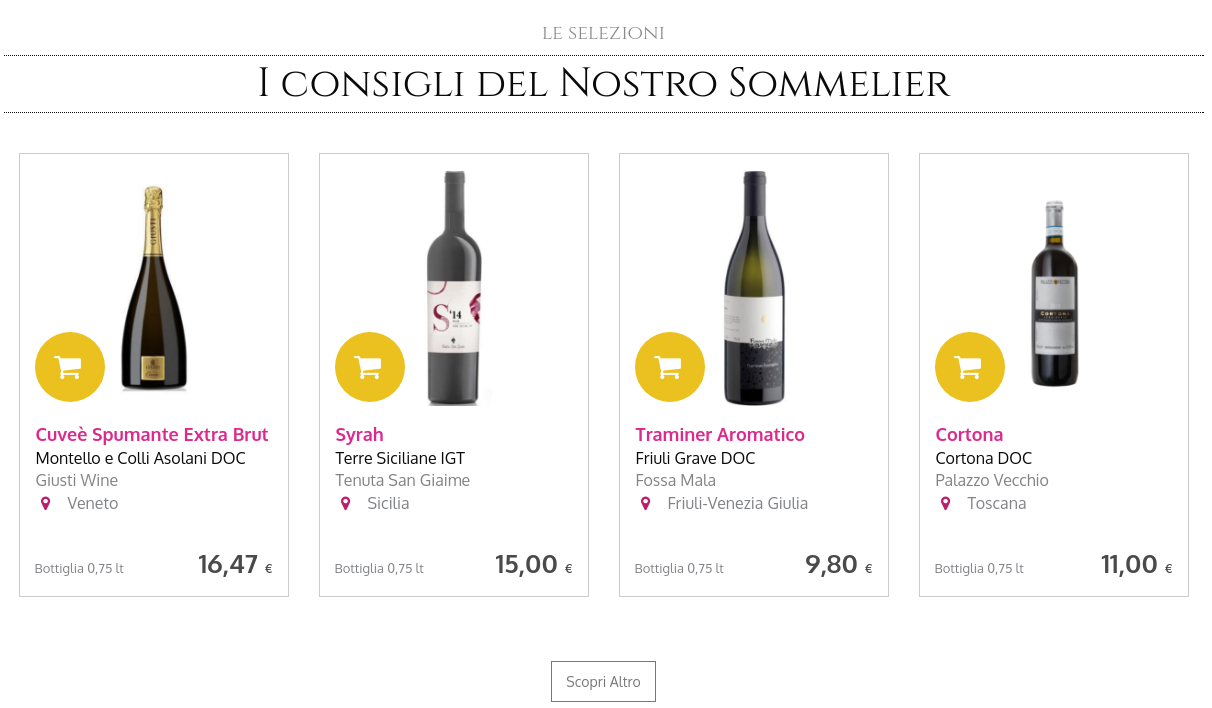
\includegraphics[width=\textwidth]{figure/oprod.png}
  \caption{Contenuto mostrato dal Widget "Origni - Slider prodotti".}
  \label{fig:oprod}
\end{figure}


% ---------------- Origini - Banda tuttoschermo ----------------
\newpage
\section{Origini - Banda tuttoschermo}
Il Widget "Origini - Banda tuttoschermo" visualizza quella porzione di HTML
usata attualmente per lo "Speciale regione" (vedi Figura \ref{fig:oreg}).

Il form permette di modificare i seguenti campi (riferirsi a Figura \ref{fig:oreg}):
\begin{itemize}
\item Sottotitolo: il testo "Speciale regione"
\item Titolo: il testo "Lombardia e cultura del buon vino"
\item Descrizione: il testo della descrizione "La varietà dei territori..."
\item Link: l'URL a cui punta il tasto \emph{Scopri Altro}
\item Image-Link: l'URL dell'immagine di sfondo
\end{itemize}

\begin{figure}
  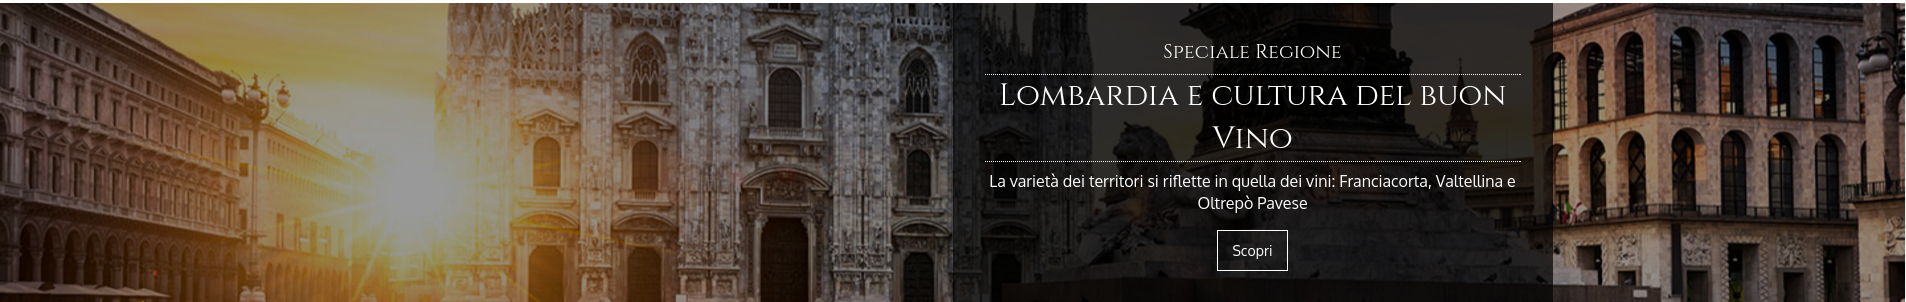
\includegraphics[width=\textwidth]{figure/oreg.png}
  \caption{Contenuto mostrato dal Widget "Origni - Banda tuttoschermo".}
  \label{fig:oreg}
\end{figure}

% ---------------- Origini - Speciale ----------------
\newpage
\section{Origini - Speciale}
Il Widget "Origni - Speciale" visualizza quella porzione di HTML
usata attualmente per lo "Speciale del mese" (vedi Figura \ref{fig:ospec}).

Il form permette di modificare i seguenti campi (riferirsi a Figura \ref{fig:ospec}):
\begin{itemize}
\item Sottotitolo: il testo "La cantina del mese"
\item Titolo: il testo "Federico Ferrero"
\item Descrizione: il testo della descrizione "L’azienda agricola Ferrero nasce..."
\item Link: l'URL a cui punta il tasto \emph{Scopri Altro}
\item Image-Link: l'URL dell'immagine da visualizzare
\end{itemize}

\begin{figure}
  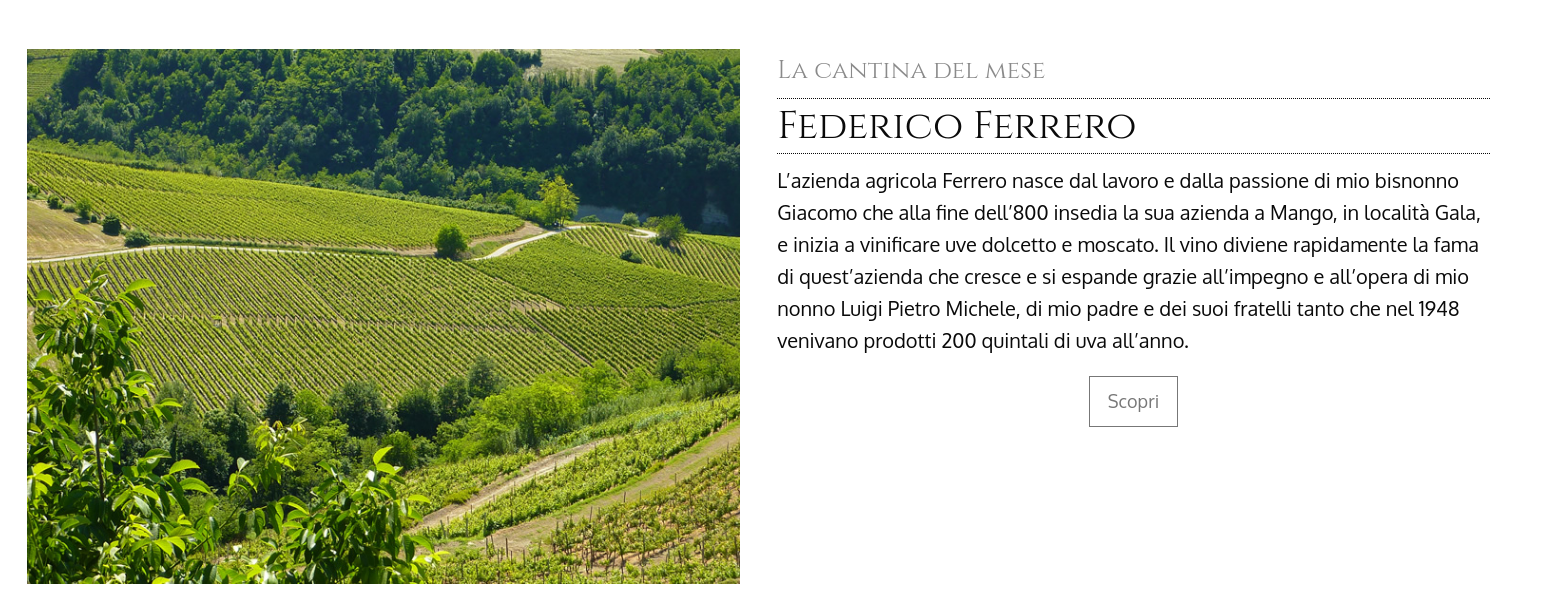
\includegraphics[width=\textwidth]{figure/ospec.png}
  \caption{Contenuto mostrato dal Widget "Origni - Speciale".}
  \label{fig:ospec}
\end{figure}

% ---------------- Origini - Accessori ----------------
\newpage
\section{Origini - Accessori}
Il Widget "Origni - Accessori" visualizza quella porzione di HTML
che mostra una lista di accessori per il vino, venduti su \url{www.kirivo.it} (vedi Figura \ref{fig:access}).

Il form permette di modificare i seguenti campi (riferirsi a Figura \ref{fig:access}):
\begin{itemize}
\item Sottotitolo: il testo "La vertina di Kirivo.it"
\item Titolo: il testo "Accessori per il vino e per la tua tavola"
\item Ids prodotti: la lista degli ID dei prodotti di Kirivo da visualizzare separati da virgola
\item Link: il teso del bottone \emph{Scopri tutti gli accessori}
\item URL: l'URL a cui punta il tasto \emph{Scopri tutti gli accessori}
\end{itemize}

\begin{figure}
  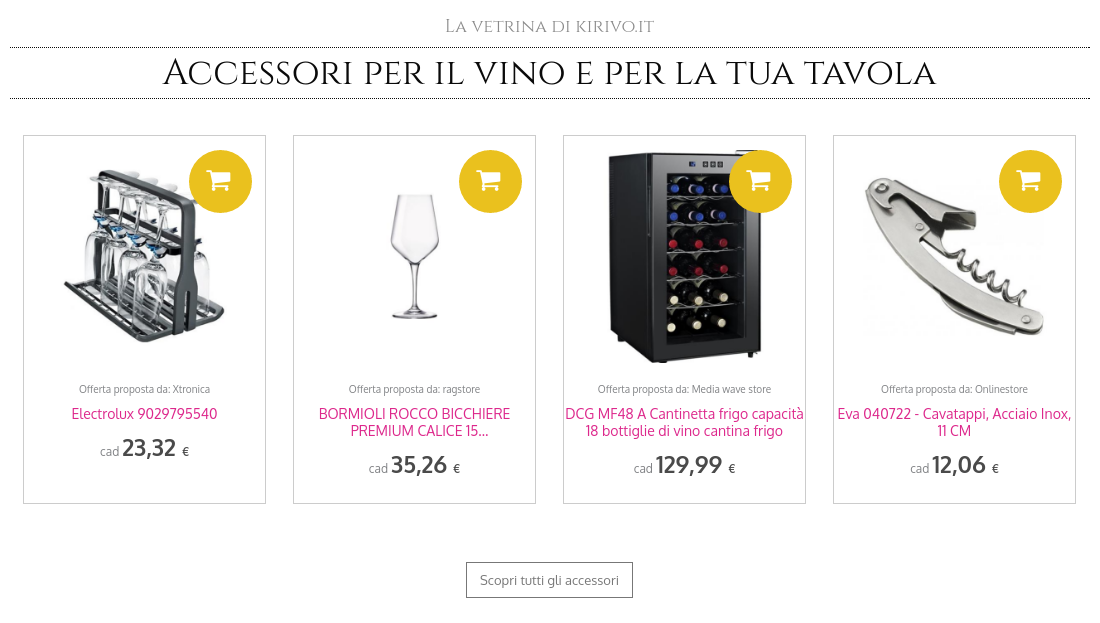
\includegraphics[width=\textwidth]{figure/access.png}
  \caption{Contenuto mostrato dal Widget "Origni - Accessori".}
  \label{fig:access}
\end{figure}

